\chapter{Homogeneous, Isotropic Cosmology}
The theory of general relativity was formulated in the previous chapter. The essence of the theory is contained in the statement given near the end of section 4.3: Spacetime is a four-dimensional manifold on which is defined a metric, $g_{ab}$, of Lorentz signature. This metric is related to the matter distribution in spacetime by Einstein's equation, $G_{ab}=8\pi T_{ab}.$

One of the most vital questions raised by the theory is: Which solution of Einstein's equation describes the spacetime we observe, i.e., which solution corresponds to our universe, or, at least, an idealized model of our universe? In order to answer this question, we first must give sufficient input via observational data and assumptions about the nature of our üniverse. Armed with this information, we may then sõlve Einstein's equation to make predictions concerning the dynamical evolution of the universe.

In this chapter, we will investigate the structure of our universe as predicted by general relativity under the assumption that the universe is homogeneous and isotropic. A precise, mathematical formulation of this assumption is given in section 5.1. The dynamical predictions of general relativity are derived in section 5.2. We discuss two important features of the homogeneous, isotropic cosmological models in section 5.3: the cosmological redshift and particle horizons. Finally, we give in section 5.4 a brief account of the history of our universe.


\section{Homogeneity and Isotropy}
\section{Dynamics of a Homogeneous, Isotropic Universe}
\section{The Cosmological Redshift; Horizons}
\section{The Evolution of Our Universe}

% \includepdf[pages=43-51]{document}